\section{Solution description} \label{Sec.SolutionDescription}

In this chapter three architectures are described. All of them involve a similar model learning approach, but differ substantially in technical details and planning algorithms. All architectures use computationally efficient latent space environment models that make predictions at a higher level of spatial abstraction, than at the level of raw pixel observations. Such models substantially reduce the amount of computation required to make predictions, as future states can be represented much more compactly. In order to increase model accuracy and robustness, all models explicitly model uncertainty in state transitions using stochastic nodes \cite{Algo.FastGenerativeModels}.
The goal stays the same: train a sufficiently accurate latent space environment's dynamics model, or such that accurately predicts future latent states and rewards to predefined cut-off point in time, and use it to plan and solve the environment. Those architectures, and experiments carried out on them, present evolution of ideas towards this goal. \\
Before all of that, the code architecture and the framework that was created to accelerate this research are described.

\subsection{HumbleRL framework}

Reinforcement Learning scientists tend to write the entire code from scratch by themselves, instead of using existing RL frameworks. This is justified by the fact, that the commonly available frameworks are not flexible enough for intended experiments or require a specific backend like TensorFlow, which might be disfavored.
HumbleRL \cite{Code.HRL} was created with this problem in mind. Its simple API allows to perform a variety of RL experiments without any restrictions on the algorithms used. Since the backend is not tied to any specific technology, it is possible to mix different neural network frameworks or not use them at all. HumbleRL provides the boilerplate code of RL loop in fig.\ref{Fig.RL} and determines the common interfaces between an agent and an environment, the rest is designed by the user.

\subsubsection{Architecture}

Framework architecture is depicted in fig. \ref{Fig.HRL_architecture}. An agent is represented by the Mind class. The Mind encapsulates action planning logic and provides it via the plan method. In order to learn, the agent acts in an environment represented by the Environment class. The Environment provides methods for resetting, taking steps, rendering and getting information about the environment. The framework includes a factory function that creates and returns e.g. wrapped OpenAI Gym environment. The agent is not usually presented with raw environment observations. Instead, it looks at states preprocessed by the Interpreter. Different interpreters can be joined together with the ChainInterpreter class. It acts as a preprocessing pipeline, with each subsequent interpreter using the output of a previous one as an input.

\begin{figure}[H]
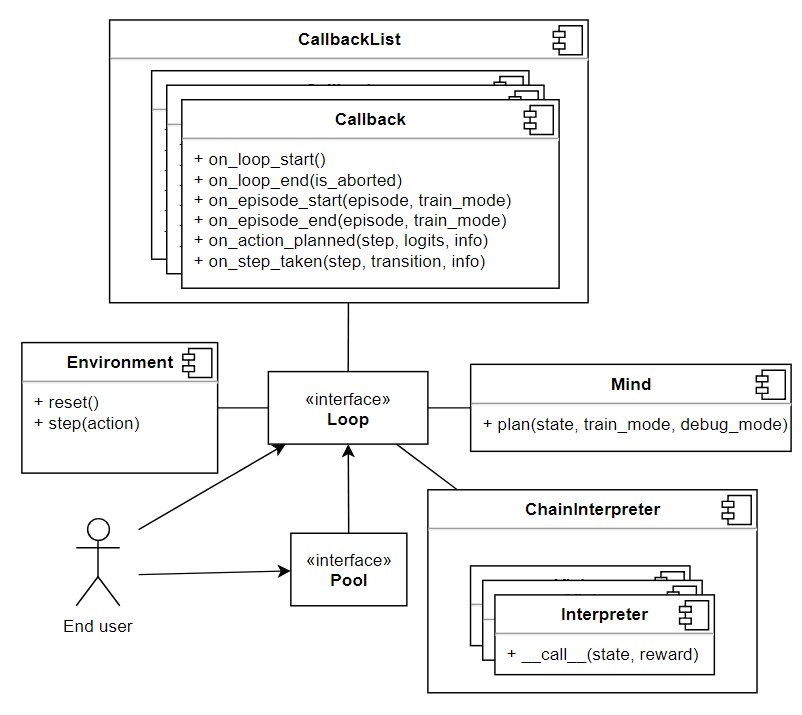
\includegraphics[width=0.6\textwidth,keepaspectratio]{figures/HumbleRL/architecture.png}
\caption{HumbleRL architecture}
\label{Fig.HRL_architecture}
\end{figure}

Framework user does not need to call all of those methods directly, those are utilized by the loop function. This function gets an action from the Mind, executes it in the Environment and then next observation is preprocessed with the Interpreter in preparation for the next step. To extend basic loop functionality, user can define callbacks that implement the Callback interface. Callbacks can react to events:
\begin{itemize}
\item at the beginning and ending of the loop,
\item at the beginning and ending of each episode,
\item after action is planned by the Mind,
\item after step is taken in the Environment.
\end{itemize}
Callbacks are accumulated in the CallbackList. The entire loop function logic is shown in fig. \ref{Fig.HRL_loop}.
Parallel version of loop function is available as the pool function. It uses predefined number of workers to execute a pool of Minds in their own Environments in parallel.

\begin{figure}[H]
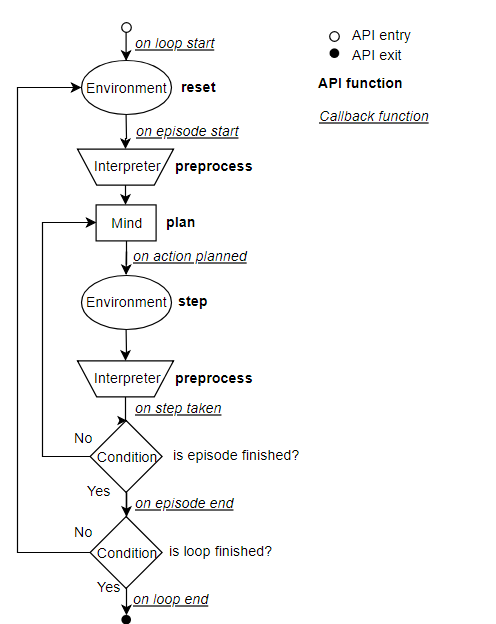
\includegraphics[width=0.6\textwidth,keepaspectratio]{figures/HumbleRL/loop.png}
\caption{HumbleRL loop function overview}
\label{Fig.HRL_loop}
\end{figure}

World Models and AlphaZero implementations use this framework and can be joined together into one architecture.

\subsection{Original World Models}

This section describes the original World Models \cite{Algo.WorldModels} algorithm which uses a learned model to create abstract task representation which, in turn, is used to solve the task by a lightweight controller. This architecture will be coupled with the AlphaZero which uses the learned model to simulate experience in the next section.

\subsubsection{World model}

A simple model inspired by human cognitive system is used. In this model, an agent has a visual sensory module that compresses observations into a small representative code. It also has a memory module that makes predictions about future codes based on historical information. Finally, the agent has a decision-making component, called the controller module, that decides what actions to take based only on the representations created by its vision and memory modules. \\
This architecture allows for training of a large neural network to tackle RL tasks by dividing the agent into a large world model and a small controller model. First a large neural network learns to model the agent’s environment in an unsupervised manner, and only then the smaller controller focuses on the credit assignment problem on a smaller search space of controller's parameters, while not sacrificing capacity and expressiveness via the larger world model.

An environment provides the agent with a high dimensional input observation at each time step. It is a 2D image frame that is part of a video sequence. The vision module role, as already mentioned, is to learn an abstract representation of each observed input frame. It uses a simple Variational Autoencoder \cite{Algo.VAE} and, as described in details in theoretical background chapter, is trained to encode each frame into low dimensional latent vector by minimizing the difference between a given frame and the reconstructed version of the frame produced by the decoder. \\
The Memory module purpose is to compress the information what happens over time in its hidden state and enable simulation of the environment. To do this, it is trained to model environment's dynamics, predicting a future latent state from history of previous latent states, as a mixture of Gaussians. It models latent states with probability distribution to model uncertainty in the environment, but also create more robust environment's representation \cite{Algo.FastGenerativeModels}. Uncertainty can originate not only from fundamental stochastic nature of the environment, but also partial observability. \\
The model is implemented as a recurrent neural network with the Mixture Density Network (MDN) on top of a RNN's hidden state. In literature this architecture is called MDN-RNN \cite{Algo.MDNRNN}. It will be further referred to as the stochastic Memory module.


Figure \ref{Fig.WorldModelsPGM} depicts the world model, the Vision and Memory modules interconnection, in graphical form. More specifically, the world model components are:
\begin{itemize}
\item Deterministic hidden state model:      $h_t = f(h_{t-1}, z_{t}, a_{t})$
\item Stochastic latent state model:         $z_{t+1} \sim p(z_{t+1}|h_t) = \sum_c\pi_c(h_t)p(z_{t+1}|h_t, c)$
\item Observation model (decoder):           $o_t \sim p(o_t|z_t)$
\item Approximate state posterior (encoder): $z_t \sim q(z_t|o_t)$
\end{itemize}
where $o$, $z$ and $a$ are high-dimensional observations, latent states and actions respectively. $f(h_{t-1}, z_{t}, a_{t})$, the hidden state model, is implemented as a recurrent neural network and $h_t$ is its hidden state. The latent state model is a mixture of Gaussians with mean and variance parameterised by a feed-forward neural network. $c$ is a mixture's component and $\pi(h)$ is a normalized vector of mixing coefficients as a function of the RNN's hidden state. The observation model is Bernoulli distribution parameterised by a deconvolutional neural network. Since the model is non-linear, directly computing the state posteriors is intractable. Instead, an encoder $q$ is used to infer approximate state posteriors from past observations and actions, where $q(s_t | h_t, o_t)$ is a diagonal Gaussian with mean and variance parameterised by a convolutional neural network followed by a feed-forward neural network.

\begin{figure}[H]
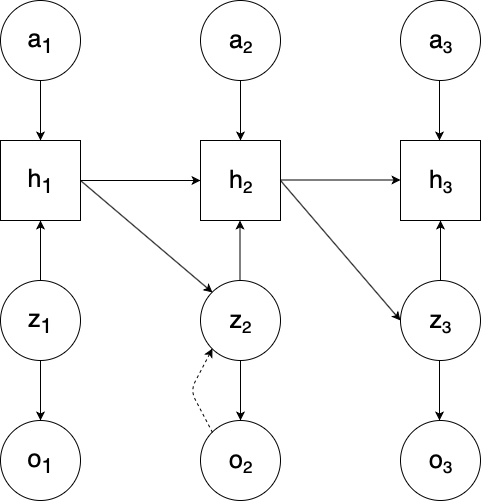
\includegraphics[width=0.45\textwidth,keepaspectratio]{figures/WorldModels/prob_graph_model.png}
\caption[World Models probabilistic graphical model]{World Models probabilistic graphical model: solid arrows describe the predictive model, dotted arrow describes the inference model, stochastic nodes are circles and squares depict deterministic nodes.}
\label{Fig.WorldModelsPGM}
\end{figure}

\subsubsection{Controller}

The Controller module is responsible for determining the course of actions to take in order to maximize the expected cumulative reward of the agent during an episode in the environment. Because it bases its decisions on abstract environment representation, learnt by the Vision and Memory modules, it can be deliberately made as simple and small as possible and trained separately from Vision and Memory modules, so that most of the agent’s complexity resides in the world model. The Controller module is a simple single layer linear model that maps a features vector constructed from latent state of the Vision module $z$ and hidden state of the Memory module $h$ directly to action $a$ at each time step:

$$a_t = W_c[z_t\,h_t] + b_c$$

where $W_c$ and $b_c$ are Controller's weights matrix and biases vector that maps the concatenated features vector $[z_t\,h_t]$ to the output action vector $a_t$. The action vector is $|A|$-dimensional, where $|A|$ is number of legal actions in an environment. It encodes predicted score of each action in the state and is used to decide which action to choose in the environment. Maximum action is taken, which means that greedy policy is used. It is true for training and testing phases. Because evolutional strategy algorithm is used for training, it doesn't impair exploration which is done on parameters level.

\subsubsection{Data collection}

To train Vision and Memory modules first collection of 10,000 random rollouts of the environment are gathered to create a dataset. An agent is acting randomly to explore the environment multiple times and records the random actions taken and the resulting observations from the environment.
This dataset is used to train the Vision module. Next, it is used to process each frame into its latent state to prepare a dataset for the Memory module training, which works entirely in the latent space.

The Controller module is trained using evolutional strategy which rollouts the environment in each epoch to evaluate population.

\subsubsection{Preprocessing}

Each frame, before it is used for any training, is central cropped if a frame from an environment includes some kind of border which doesn't inform an agent in anyway. This operation depends on a specific environment. It is then resized to 64 x 64 pixels for all environments. All three colour channels are preserved. Actions are one-hot encoded and default 4 action repeat from OpenAI Gym \cite{Code.OpenAIGym} is used as common in reinforcement learning \cite{Algo.DQN} to reduce the planning horizon and provide a clearer learning signal to the model.

\subsubsection{Implementation details}

HumbleRL is used to implement the original World Models architecture from the paper. This allows for easy adjustments for experiments purposes and to couple the world model with AlphaZero implementation in HumbleRL. An agent exploring an environment (Mind) and a callback are used to gather transitions and save them to an external storage. The framework allows to focus strictly on collecting trajectories and not worry about agent-environment interactions. \\
Collected transitions are used to train the Vision and Memory components. The popular LSTM architecture \cite{Algo.LSTM} implements the Memory module RNN with 256 hidden units. The MDN is composed of 5 16-dimensional Gaussians with mean and log standard deviation parameterised by one layer feed-forward neural networks with linear activations. The Vision module neural networks are convolutional and deconvolutional neural networks shown in figure \ref{Fig.WorldModelsVAEArchitecture} where latent state size, $\mu$ and $\sigma$ vectors dimensionality, equals 16. \\
For Vision training Keras \cite{Code.Keras} framework is used to adjust the parameters by the stochastic gradient descent on a standard Evidence Lower Bound loss. For Memory training PyTorch \cite{Code.PyTorch} framework is used, since it is easier to work with recurrent neural networks than in Keras, to, again, adjust the parameters by the stochastic gradient descent on a negative log-probability loss of the mixture density network. HumbleRL is not constricted to work with any particular deep learning library, so it is not a problem to mix the solutions, as long as trained models are wrapped in HumbleRL's interfaces.
The Vision module is trained using the Adam optimizer \cite{Algo.Adam} with a learning rate of $10^{-3}$ and $\epsilon = 10^{−7}$ on batches of 256 images. The Memory module is trained using the Adam optimizer \cite{Algo.Adam} too with a learning rate of $10^{-3}$ and $\epsilon = 10^{−8}$ on batches of 128 sequence chunks of length 1000. \\

\begin{figure}[H]
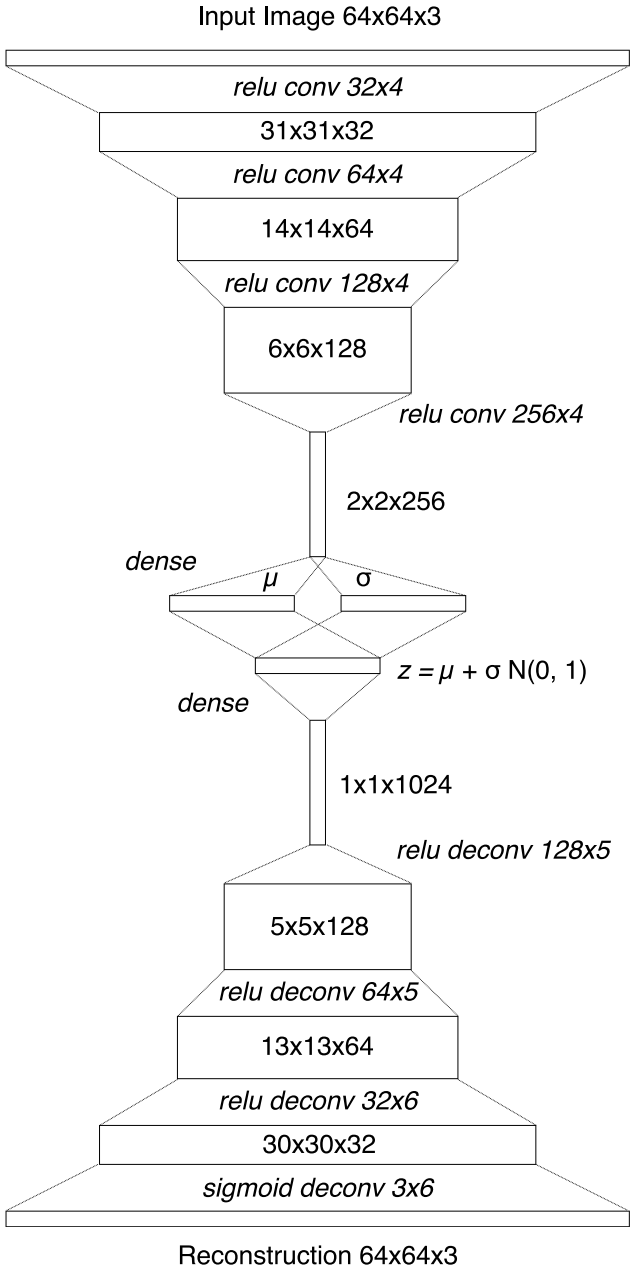
\includegraphics[width=0.45\textwidth,keepaspectratio]{figures/WorldModels/world_models_vae_architecture.png}
\caption{World Models VAE neural network architecture \cite{Algo.WorldModels}}
\label{Fig.WorldModelsVAEArchitecture}
\end{figure}

The Controller module gets a feature vector as its input, consisting of latent state $z$ and the hidden state of the MDN-RNN. In all environments, this hidden state is the output vector $h$ of the LSTM. \\
Covariance-Matrix Adaptation Evolution Strategy (CMA-ES) \cite{Algo.CMAES} is used for the Controller module training. It evolves the weights $W_c$ and biases $b_c$ of the module. A population size of 64 is used and each agent plays in the environment 5 episodes. The fitness value for the agent is the average cumulative reward of the 5 episodes.

Hyper-parameters presented are used as defaults in experiments described in the next chapter.

\subsection{World Models and AlphaZero}

World Models' agent \cite{Algo.WorldModels} successfully plans using a learned model where the model is used to generate simulated experience on which the policy is trained. This section describes attempt to adjust and utilize the world model part of the agent in the AlphaZero search algorithm. This is different application of the model than in the original paper, where only future latent states and done flag are predicted, and therefore the world model needs to be extended with a reward predictor and the controller is replaced by AlphaZero.

\subsubsection{World model}

For the world model part, Vision and Memory modules, architecture stays the same with a slight change. Because benchmarks include only deterministic environments and AlphaZero in its original form can only work with a deterministic dynamics model, this architecture use the Memory module without the MDN and with a linear model instead. In fact, it uses two linear models to output the next latent state and reward.
\begin{itemize}
\item Deterministic hidden state model:      $h_t = f(h_{t-1}, s_{t}, a_{t})$
\item Deterministic latent state model:      $z_{t+1} = f(h_t)$
\item Deterministic reward model:            $r_{t+1} = f(h_t)$
\item Observation model (decoder):           $o_t \sim p(o_t|z_t)$
\item Approximate state posterior (encoder): $z_t \sim q(z_t|o_t)$
\end{itemize}
where $f$ is the latent state model and the reward model are the linear models. It will be further referred to as the deterministic Memory module.

\subsubsection{Controller}

AlphaZero \cite{Algo.AlphaZero} is very similar to the MCTS algorithm, explained in the chapter \ref{Sec.TheoreticalBackground}. The selection and evaluation phases are modified though. AlphaZero uses policy and value networks to guide its search. Each edge in the search tree, $(s, a, s')$ where $s$ is a state, $a$ is an action and $s'$ is the next state, stores a prior probability of choosing it $P(s, a)$, a visit count $N(s, a)$, an action-value $Q(s, a)$ and a reward $R(s, a, s')$ of transition represented by this edge. Each simulation starts from the root state, $s_t$ at depth or time step $t=0$, and iteratively selects moves that maximise an upper confidence bound $Q(s, a) + U(s, a)$, where $U(s, a) \propto P(s, a)/(1+ N(s, a))$ \cite{Algo.AlphaGoZero}, until a leaf node is encountered. This leaf position is expanded by the world model to generate both the next state and reward, $s_{t'}$ and $r_{t'}$ at depth or time step $t'$, and evaluated by the networks to generate both prior actions probabilities and its value, $P(s_{t'}, \cdot)$ and $V(s_{t'})$. Each edge traversed in the simulation is updated to increment its visit count $N(s_t, a_t)$, and to update its action-value to the mean evaluation over these simulations:

$$Q(s_t, a_t) = 1/N(s_t, a_t) \sum_{t'}\Big[ \sum^{t'}_{i = t + 1}r_i + V(s_{t'}) \Big]$$

Figure \ref{Fig.MCTSinAlphaZero} depicts this process. After multiple simulations, which could be stopped after the absolute number of simulations or after timeout, the result is a vector of search probabilities recommending moves to play, $\boldsymbol\pi$, proportional to the visit count for each move, $\pi_a \propto N(s, a)$. How these are used to choose an action to take by the agent is discussed in the next section.

\begin{figure}[H]
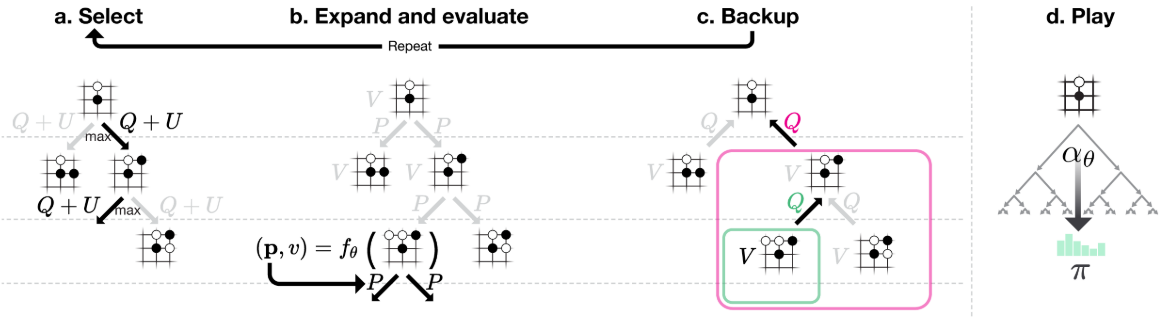
\includegraphics[width=0.9\textwidth,keepaspectratio]{figures/AlphaZero/MCTS.png}
\caption{Monte-Carlo tree search in AlphaZero \cite{Algo.AlphaGoZero}}
\label{Fig.MCTSinAlphaZero}
\end{figure}

\subsubsection{Implementation details, data collection and preprocessing}

The world model implementation details, preprocessing and data collection for Vision and Memory modules are the same as in the original World Models. The world model latent state size is 16 and the LSTM hidden size is 256. Input to value and policy networks is the same concatenated features vector of latent and hidden states, $[z_t\,h_t]$.

The AlphaZero controller uses the world model for simulations. The Vision module is used as the Interpreter which encodes incoming observations into latent space. The Memory module, wrapped in the MDP interface from HumbleRL, is used in the expansion phase of AlphaZero. The Mind class, which is implemented by the AlphaZero algorithm, returns actions' scores. These are actions visit counts from the root state node, which are then used to choose an action by a policy. During training actions are sampled with probability proportional to these visit counts for 12 warm-up steps at the beginning of each episode to enhance exploration and after warm-up a greedy policy is used. During testing always greedy policy is used, which picks an action which was visited most often.
Pseudo-code written in Python of the search algorithm in the Mind is shown below:

\noindent\begin{minipage}{\textwidth} % This ensures that the code block won't be dividend between two pages.
\begin{lstlisting}[language=Python]
def plan(self, state):
    # Get/create root node
    root = self.query_tree(state)

    # Perform simulations
    simulations = 0
    start_time = time()
    while time() < start_time + self.timeout and simulations < self.max_simulations:
        # Simulate
        simulations += 1
        leaf, path = self.simulate(root)

        # Expand and evaluate
        value = self.evaluate(leaf)

        # Backup value
        self.backup(path, value)

    # Get actions' visit counts
    actions = np.zeros(self.model.action_space.num)
    for action, edge in root.edges.items():
        actions[action] = edge.num_visits

    return actions
\end{lstlisting}
\end{minipage}

AlphaZero value and policy networks are two linear models trained by reinforcement learning from self-play games, starting from randomly initialized parameters. Each game is played by running the search, described above, at each position, $s$, and then selecting a move either proportionally (for exploration) or greedily (for exploitation) according to returned move probabilities, which are normalised visit counts at the root state, $\boldsymbol\pi$. These search probabilities usually select much stronger moves than the raw move probabilities of the policy network. The MCTS search may therefore be viewed as a powerful policy improvement operator \cite{Book.RLAI}. Self-play with search – using the improved MCTS-based policy to select each move by the agent, then using the game cumulative reward, or the return, as a sample of the value at each time step – may be viewed as a powerful policy evaluation operator. The main idea of this reinforcement learning algorithm is to use these search operators repeatedly in a policy iteration framework \cite{Algo.AlphaGoZero}. The linear models' parameters are updated to make the move probabilities and values more closely match the improved search probabilities and self-play cumulative rewards at each step. These new parameters are used in the next iteration of self-play to make the search even stronger. \\
The agent's experience and score statistics used for training are gathered using callbacks during the self-play phase. Maximum of 1000 latest games are kept. The models training phase takes place after 10 self-play games and lasts for 5 epochs. The training phase is performed using the Keras \cite{Code.Keras} framework. Specifically, the parameters are adjusted by the stochastic gradient descent on a loss function that sums over mean squared errors of the value network, cross-entropy losses of the policy network and L2 weights regularization scaled by a factor of $10^{-4}$ in batches of 256 examples, where each example is a features vector of a state, a value sample from self-play and a MCTS action probabilities vector. The Nesterov's momentum optimizer \cite{Algo.Nesterov} is used with a learning rate of $10^{-2}$ and a momentum of $0,9$.

Hyper-parameters presented are used as defaults in experiments described in the next chapter.

\subsection{PlaNet}

PlaNet (Deep Planning Network) \cite{Algo.PlaNet} shows working example of a planning agent that searches for the best sequence of future actions using a learned model in continuous control tasks. This is close to what this work tries to accomplish, but for a different type of environments. This section describe how it was utilized in episodic discrete tasks.

\subsubsection{World model}

This architecture uses recurrent state space model (RSSM) which is similar to what World Models does. This latent dynamics model is designed with both deterministic and stochastic components \cite{Algo.FastGenerativeModels}. Original experiments indicate having both components to be crucial for high planning performance. It also uses a generalized variational bound that include multi-step predictions. Using only terms in latent space results in a fast regularizer that can improve long-term predictions \cite{Algo.PlaNet}.

Same as in World Models, the model is provided with image observations. It even uses the same Variational Autoencoder with the same neural network architecture to encode the observations into latent space. The difference lies in the dynamics model shown in figure \ref{Fig.PlaNetPGM} with following components:
\begin{itemize}
\item Deterministic hidden state model:      $h_t = f(h_{t-1}, s_{t-1}, a_{t-1})$
\item Stochastic latent state model:         $s_t \sim p(s_t|h_t)$
\item Observation model (decoder):           $o_t \sim p(o_t|h_t, s_t)$
\item Reward model:                          $r_t \sim p(r_t|h_t, s_t)$
\item Approximate state posterior (encoder): $s_t \sim q(s_t|o_{\leqslant t}, a_{< t}) = \prod_{i=1}^tq(s_t|h_t,o_t)$
\end{itemize}
where $o$, $s$ and $a$ are high-dimensional observations, latent states and actions respectively. $f(h_{t-1}, s_{t-1}, a_{t-1})$, the deterministic state model, is implemented as a recurrent neural network and $h_t$ is its hidden state. The latent state model is Gaussian with mean and variance parameterised by a feed-forward neural network, the observation model is Gaussian with mean parameterised by a deconvolutional neural network and identity covariance, and the reward model is a scalar Gaussian with mean parameterised by a feed-forward neural network and unit variance. Since the model is non-linear, directly computing the state posteriors is intractable. Instead, an encoder $q$ is used to infer approximate state posteriors from past observations and actions, where $q(s_t | h_t, o_t)$ is a diagonal Gaussian with mean and variance parameterised by a convolutional neural network followed by a feed-forward neural network.

\begin{figure}[H]
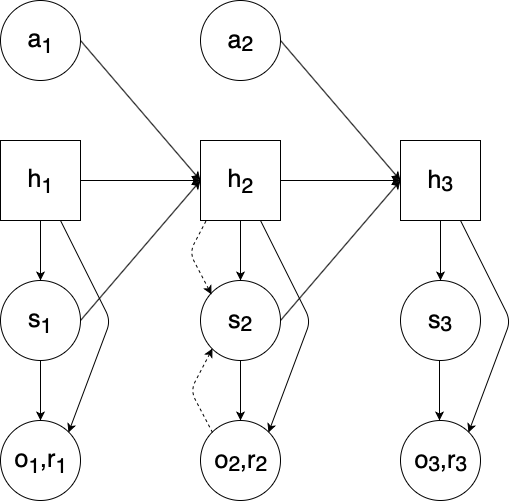
\includegraphics[width=0.45\textwidth,keepaspectratio]{figures/PlaNet/prob_graph_model.png}
\caption[World Models probabilistic graphical model]{PlaNet probabilistic graphical model: solid arrows describe the predictive model, dotted arrow describes the inference model, stochastic nodes are circles and squares depict deterministic nodes.}
\label{Fig.PlaNetPGM}
\end{figure}

\noindent There are two deviations from the World Models architectures:
\begin{itemize}
\item Hidden states are ``shifted'' to the right, so the previous state and action are used to predict the current hidden state $h$ and it is then used to predict the current latent state $s$.
\item VAE's decoder and encoder (named Vision in World Models) use the dynamics model's hidden state for prediction and inference. This way the likelihood and the posterior are conditioned on past observations too, as opposed to World Models.
\end{itemize}

Intuitively, this model can be understood as splitting the state into a stochastic part and a deterministic part, which depend on the stochastic and deterministic parts at the previous time step through the RNN. Importantly, all information about the observations must pass through the sampling step of the encoder to avoid a deterministic shortcut from inputs to reconstructions.

\subsubsection{Planner}

The agent plans using the cross entropy method (CEM) \cite{Algo.CEM} to search for the best action sequence under the model. CEM is a population-based optimization algorithm that infers a distribution over action sequences that maximize the objective.
First, a time-dependent diagonal Gaussian belief over optimal action sequences gets initialized: $a_{t:t+H} \sim Normal(\mu_{t:t+H}, \sigma^2_{t:t+H}I)$, where $t$ is the current time step of the agent and $H$ is the length of the planning horizon. Starting from zero mean and unit variance, it is used to sample candidate action sequences. To evaluate a candidate action sequence under the learned model a trajectory starting from the current state is sampled by the model using the action sequence as an input and the predicted rewards are summed along the sequence. This sum is used as the action sequence fitness score. Since it is a population-based optimizer, it is sufficient to consider a single trajectory per action sequence and thus focus the computational budget on evaluating a larger number of different sequences. Then, the belief gets re-fitted to the best sequences and next optimization iteration starts the same way. At the end, the planner returns the mean of the belief for the current time step $\mu_t$ which is then used by the policy to choose discrete action. Importantly, after receiving the next observation, the belief over action sequences starts from zero mean and unit variance again to avoid local optima. \\
Because the reward is modeled as a function of the latent state, the planner can operate purely in latent space without generating images, which allows for fast evaluation of large batches of action sequences. The algorithm is presented in the figure \ref{Fig.CEMinPlaNet} below.

\begin{figure}[H]
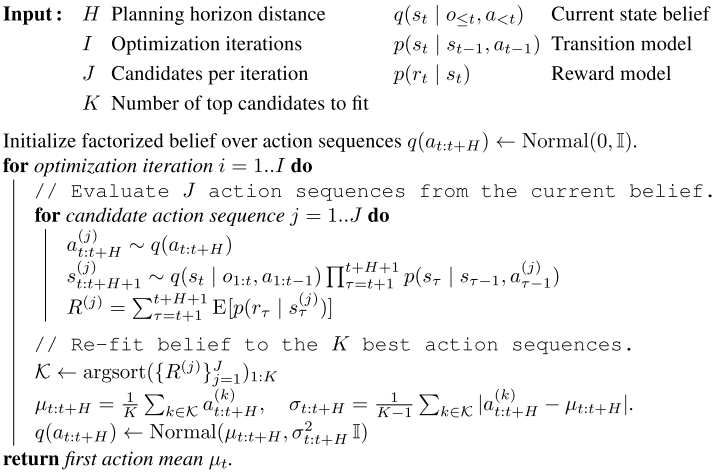
\includegraphics[width=0.9\textwidth,keepaspectratio]{figures/PlaNet/CEM.png}
\caption{Latent planning with CEM \cite{Algo.PlaNet}}
\label{Fig.CEMinPlaNet}
\end{figure}

\subsubsection{Data collection}

Since the agent may not initially visit all parts of the environment, the data-aggregation iterative method described in section \ref{Sec.ModelLearning} is used. Starting from a small amount of 6 seed episodes collected under random actions, the model is trained and one additional episode is added to the data set every 5000 update steps.

\subsubsection{Preprocessing}

Each image gets preprocessed by reducing the bit depth to 5 bits as in \cite{Algo.Glow5bit}. It is then resized to 64 x 64 pixels for all environments.
Actions are one-hot encoded and each action gets repeated 4 times as common in reinforcement learning \cite{Algo.DQN} to reduce the planning horizon and provide a clearer learning signal to the model.

\subsubsection{Implementation details}

This time official code from repository \cite{Code.PlaNet} was adjusted and used for experiments. The code architecture follows principles from other PlaNet author's paper \cite{Code.TFAgents}.
The RSSM uses a GRU \cite{Algo.GRU} with 200 units as deterministic path in the dynamics model and implements all other functions as two fully connected layers of size 200 with ReLU activations \cite{Algo.ReLU}. Distributions in latent space are 30-dimensional diagional Gaussians with predicted mean and standard deviation.
The observation model and the approximate state posterior are implemented with the Variational Autoencoder, the same as in World Models (see fig.\ref{Fig.WorldModelsVAEArchitecture}). The reward model is implemented with a feed-forward neural network with two hidden layers of size 100.
The model is trained jointly using the Adam optimizer \cite{Algo.Adam} with a learning rate of $10^{-3}$ and $\epsilon = 10^{−4}$, and gradient clipping norm of 1000 on batches of 50 sequence chunks of length 50. The KL divergence terms are also scaled relatively to the reconstruction terms and the model is granted free nats by clipping the divergence loss below this value. Both parameters are tuned in the experiments chapter. The latent overshooting from the paper \cite{Algo.PlaNet} is used with overshooting KL divergence terms additionally scaled by a factor of $1/50$. \editnote{QUESTION: Should we rewrite here full loss? It's quite enormous and complicated. Reader can check it in the PlaNet's paper.}

Planner uses planning horizon of 12, which means that it evaluates 12 actions in the future. Starting from zero mean and unit variance, 1000 candidate action sequences are sampled and evaluated under the learned model. Then the belief gets re-fitted to the top 100 action sequences with the highest fitness scores. After 10 iterations, the planner returns the mean of the belief for the current time step $\mu_t$ which is then used by the policy to choose discrete action. When collecting episodes for the training data set the epsilon greedy policy is used with $\epsilon = 0,3$. During test phase the greedy policy is used, which chooses the action that maximises the returned belief.

Hyper-parameters presented are used as defaults in experiments described in the next chapter.
